\subsubsection{Example}

    \begin{itemize}[noitemsep,topsep=0pt]
      \item Starting position: (0.0, -4.0, 32.0)
      \item End position: (0.0, -2.0, 7.0) 
      \item Euclidean distance from the object: 7.280109889280518
      \item Object can be seen: True
      \item Success: True
      \item Object type: a campsite
      
    \end{itemize}
    

    \begin{center}
    \includegraphics[width=0.7\linewidth]{images/Sonnet-ForestNew/25_r0_.pdf}
    \end{center}
    

    \begin{center}
    \includegraphics[width=0.7\linewidth]{images/Sonnet-ForestNew/25_r0__sit_awareness.pdf}
    \end{center}
    

    \begin{drama}
    \Character{Benchmark}{re}
    \Character{Claude 3.5 Sonnet}{gpt}
    
\respeaks: \( < \)Context\( > \)
    You are in command of a UAV, tasked with finding a campsite.
\( < \)/Context\( > \) \texttt{(REST OF THE PROMPT)}
\respeaks: Image 1:
\StageDir{\re{} presents \gpt{} with a relevant image}

    \begin{center}
    
\includegraphics[width=0.5\linewidth]{images/Sonnet-ForestNew/25_r0__0.jpg}
    \end{center}
    
\respeaks: Your current altitude is 32 meters above ground level.
\gptspeaks: \( < \)Reasoning\( > \)I can see what appears to be a tent or small campsite near the center of the image. To get a better view and position myself correctly, I'll move to coordinates (0, 0) which appear to be directly above the campsite. Since I need to be below 10 meters to confirm the target, I'll also decrease my altitude by 25 meters, bringing me to approximately 7 meters above ground level.\( < \)/Reasoning\( > \)
\( < \)Action\( > \)(0, 0, -25)\( < \)/Action\( > \)
\respeaks: Image 2:
\StageDir{\re{} presents \gpt{} with a relevant image}

    \begin{center}
    
\includegraphics[width=0.5\linewidth]{images/Sonnet-ForestNew/25_r0__1.jpg}
    \end{center}
    
\respeaks: Your current altitude is 7 meters above ground level.
\gptspeaks: \( < \)Reasoning\( > \)I can now clearly see the campsite. I'm at the correct altitude (7 meters, which is below 10 meters) and I'm centered on the target area. The campsite is clearly visible in my field of view.\( < \)/Reasoning\( > \)
FOUND
\end{drama}
\subsubsection{Example}

    \begin{itemize}[noitemsep,topsep=0pt]
      \item Starting position: (-8.0, 20.0, 54.0)
      \item End position: (-1.0, 0.0, 8.0) 
      \item Euclidean distance from the object: 8.06225774829855
      \item Object can be seen: True
      \item Success: True
      \item Object type: a trash pile
      
    \end{itemize}
    

    \begin{center}
    \includegraphics[width=0.7\linewidth]{images/Sonnet-ForestNew/26_r0_.pdf}
    \end{center}
    

    \begin{center}
    \includegraphics[width=0.7\linewidth]{images/Sonnet-ForestNew/26_r0__sit_awareness.pdf}
    \end{center}
    

    \begin{drama}
    \Character{Benchmark}{re}
    \Character{Claude 3.5 Sonnet}{gpt}
    
\respeaks: \( < \)Context\( > \)
    You are in command of a UAV, tasked with finding a trash pile.
\( < \)/Context\( > \) \texttt{(REST OF THE PROMPT)}
\respeaks: Image 1:
\StageDir{\re{} presents \gpt{} with a relevant image}

    \begin{center}
    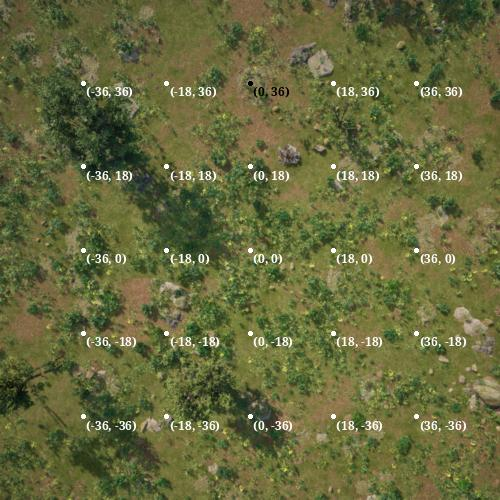
\includegraphics[width=0.5\linewidth]{images/Sonnet-ForestNew/26_r0__0.jpg}
    \end{center}
    
\respeaks: Your current altitude is 54 meters above ground level.
\gptspeaks: \( < \)Reasoning\( > \)
From this initial altitude of 54 meters, I can see a wide area but need to conduct a systematic search for the trash pile. I notice some variations in the terrain and need to get lower to better identify potential targets. I'll start by moving to the center of the visible area and descending to get a better view of any potential trash piles.
\( < \)/Reasoning\( > \)
\( < \)Action\( > \)(0, 0, -24)\( < \)/Action\( > \)
\respeaks: Image 2:
\StageDir{\re{} presents \gpt{} with a relevant image}

    \begin{center}
    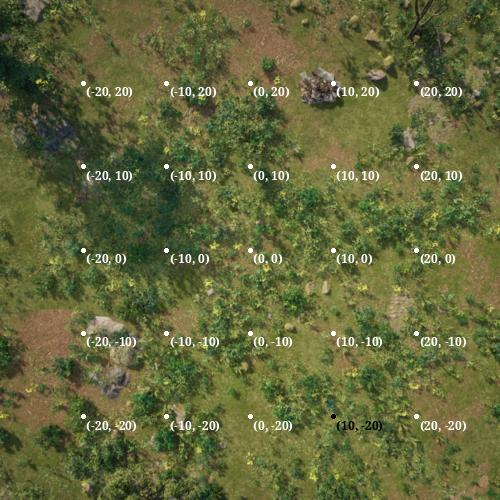
\includegraphics[width=0.5\linewidth]{images/Sonnet-ForestNew/26_r0__1.jpg}
    \end{center}
    
\respeaks: Your current altitude is 30 meters above ground level.
\gptspeaks: \( < \)Reasoning\( > \)
At 30 meters altitude, I can now see more detail but still need to search systematically. I notice what appears to be some irregular objects or potential debris near the coordinates (10, 20). I'll move in that direction and descend further to investigate more closely.
\( < \)/Reasoning\( > \)
\( < \)Action\( > \)(10, 20, -20)\( < \)/Action\( > \)
\respeaks: Image 3:
\StageDir{\re{} presents \gpt{} with a relevant image}

    \begin{center}
    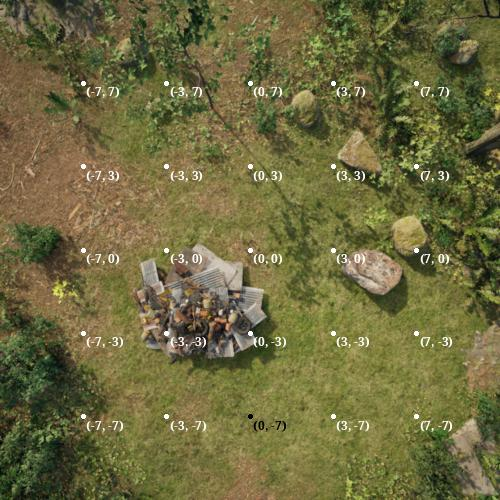
\includegraphics[width=0.5\linewidth]{images/Sonnet-ForestNew/26_r0__2.jpg}
    \end{center}
    
\respeaks: Your current altitude is 10 meters above ground level.
\gptspeaks: \( < \)Reasoning\( > \)
I can now clearly see a trash pile consisting of various debris near coordinates (-3, -3). I need to position myself directly above it and ensure I'm at the correct altitude to meet the mission requirements. I'm currently at 10 meters which is just at the maximum allowable height, but I'll descend slightly to ensure I'm definitively under 10 meters while staying centered over the trash pile.
\( < \)/Reasoning\( > \)
\( < \)Action\( > \)(-3, -3, -2)\( < \)/Action\( > \)
\respeaks: Image 4:
\StageDir{\re{} presents \gpt{} with a relevant image}

    \begin{center}
    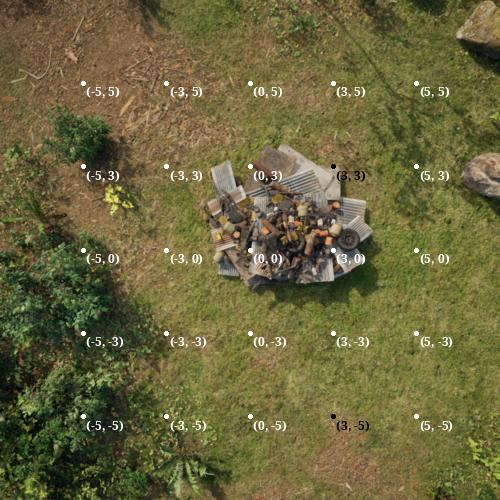
\includegraphics[width=0.5\linewidth]{images/Sonnet-ForestNew/26_r0__3.jpg}
    \end{center}
    
\respeaks: Your current altitude is 8 meters above ground level.
\gptspeaks: FOUND

\( < \)Reasoning\( > \)
I am now perfectly positioned above the trash pile at 8 meters altitude, which is below the required 10 meters. The trash pile is clearly visible in my field of view and I am centered above it. This meets all the mission requirements:
1. Below 10 meters (at 8 meters)
2. Object in field of view
3. Centered on the object
\( < \)/Reasoning\( > \)
\end{drama}
